\chapter{General Context of the Project}
\label{chap:context}

\section*{Introduction}

This chapter situates the work within its broader context. It first presents the
host organization, \textbf{Boston Consulting Group} and its technology unit
\textbf{BCG~X}, together with the product team to which I was assigned and the
internal-product model that frames the project. It then states the
confidentiality framework, and introduces the energy-transition and
\textbf{Power-to-X} context. It describes the \textbf{Energy Transition
Optimizer} and its fragile initial state, sets out the problem statement,
scoping questions, and objectives, and closes with the project-management
approach and timeline.

\section{Host Organization}

Large organizations increasingly rely on data, cloud, and artificial
intelligence to address operational challenges and unlock new sources of growth.
BCG combines management-consulting expertise with engineering and product
capabilities through BCG~X, in order to deliver digital solutions at scale. The
internship was hosted by Boston Consulting Group (BCG), within its technology
build and design unit BCG~X; the following sections present both entities, their
activities, organizational structure, and culture.

\subsection{Boston Consulting Group (BCG)}

\begin{figure}[H]
  \centering
  
\includegraphics[scale=1.2]{Logos/BCG_Logo_Monogram_Green.png}
  \caption{BCG logo.}
  \label{fig:bcg-logo}
\end{figure}

\subsubsection{History}

BCG was founded in 1963 by Bruce Henderson and is headquartered in Boston,
Massachusetts. Since its creation, the firm has built a strong reputation in
strategy consulting, business transformation, and analytical problem solving. It
now supports organizations from the private, public, and social sectors across a
broad range of industries, and its offering has progressively integrated data,
technology, and digital-transformation services.

\subsubsection{BCG at a glance}

Figure~\ref{fig:bcg-glance} summarizes the firm's publicly reported footprint.

\begin{figure}[H]
  \centering
  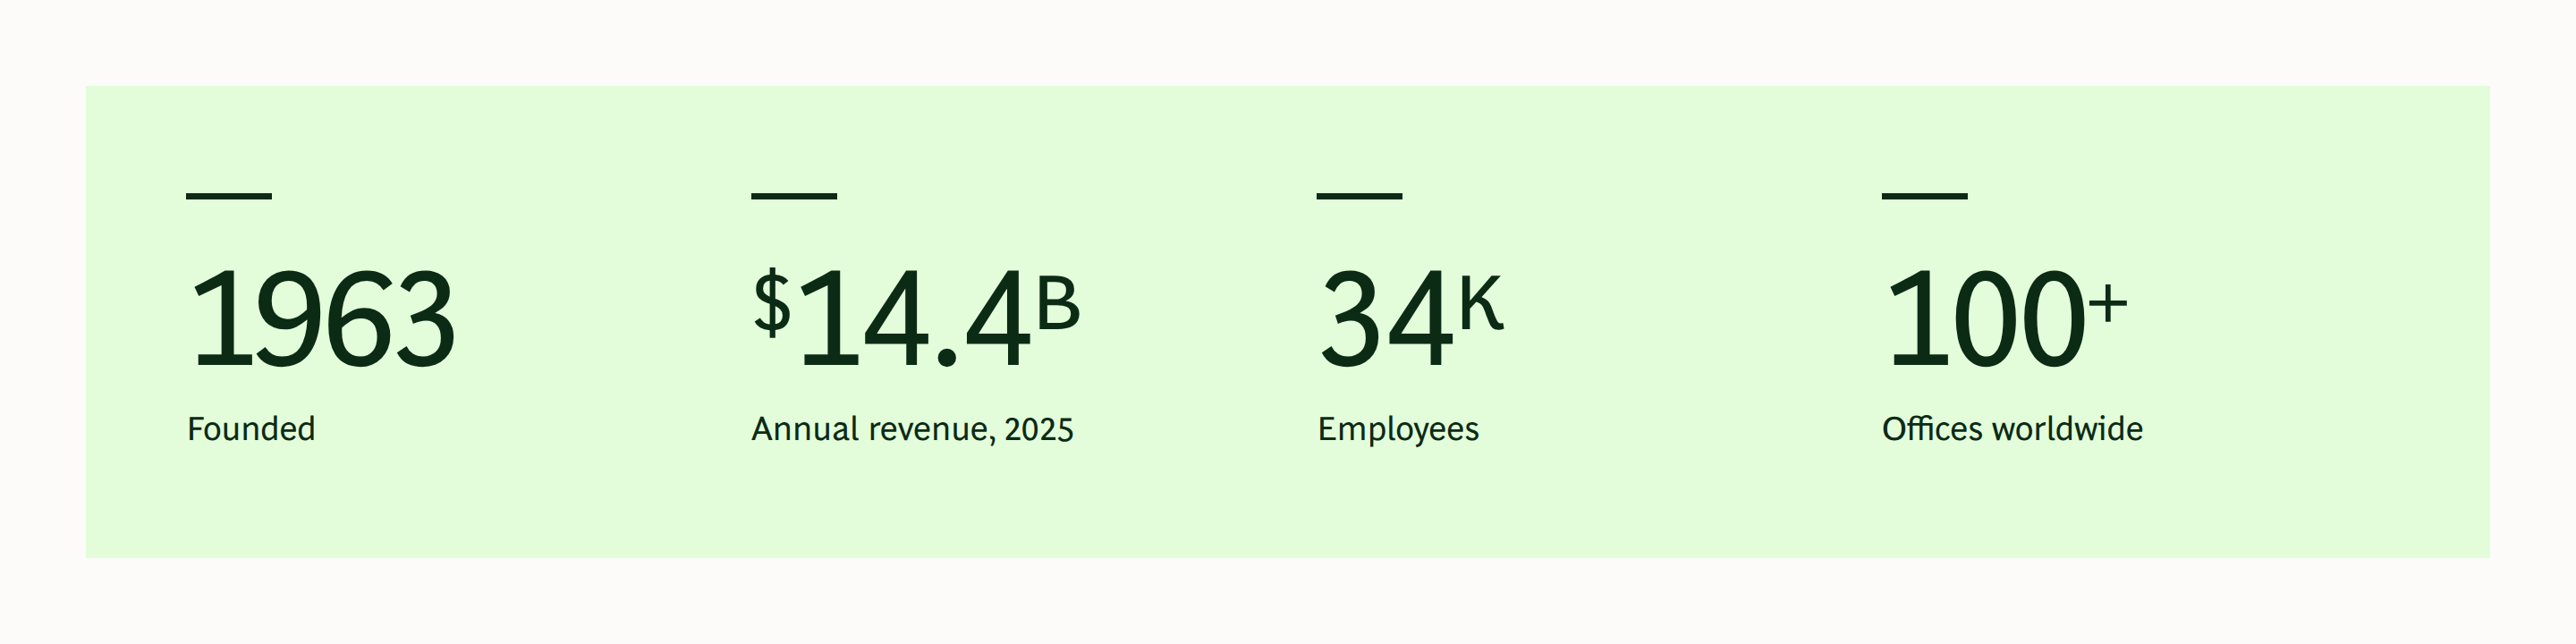
\includegraphics[width=\linewidth]{Figures/bcg-stats-light.png}
  \caption{BCG at a glance (publicly reported figures).}
  \label{fig:bcg-glance}
\end{figure}

\subsubsection{Business areas}

BCG covers business transformation, corporate strategy, digital transformation,
sustainability, mergers and acquisitions, innovation management, and operational
performance. Industry coverage includes healthcare, financial services, consumer
goods, energy, technology, and the public sector.

\subsection{BCG X}

\begin{figure}[H]
  \centering
  
\includegraphics[scale=1]{Logos/BCG_X.jpg}
  \caption{BCG X logo.}
  \label{fig:bcg-x-logo}
\end{figure}

\subsubsection{Presentation}

BCG~X is the technology, design, and build unit of BCG. It accelerates the
digital transformation of large organizations by combining engineering, data,
and design capabilities with the strategic positioning of the firm. Unlike a
traditional software vendor, BCG~X operates within the broader consulting
environment: beyond delivering software, it also helps organizations build
capabilities and adopt new technologies.

\subsubsection{Business areas}

BCG~X concentrates on four core capabilities:

\begin{itemize}
  \item \textbf{AI and Generative AI}: design and delivery of
    artificial-intelligence solutions for business functions, automation, and
    decision support.
  \item \textbf{Customer Experience for Growth}: digital strategies and customer
    journeys oriented toward growth and engagement.
  \item \textbf{Venture and Business Builds}: end-to-end support of new ventures,
    from idea to market.
  \item \textbf{Digital Platform Builds}: secure and scalable digital platforms
    supporting large-scale trans\-for\-ma\-tions.
\end{itemize}

\subsection{Organizational Structure}

BCG adopts a structured yet agile approach, promoting global collaboration
through its technology unit, BCG~X. Led by Sylvain Duranton (Global Leader) and
Jon Ferris (Chief Financial Officer), BCG~X's organizational structure includes
regional and functional leads who oversee specialized areas and regional
centers. This design ensures efficient global coordination and responsiveness to
client needs.

Each regional center (including Morocco, Germany, China, Singapore, and India) is
managed by dedicated leaders who implement localized yet globally aligned
strategies. This structured regional management facilitates effective service
delivery tailored to local market requirements while maintaining consistent
global standards.

\begin{figure}[H]
  \centering
  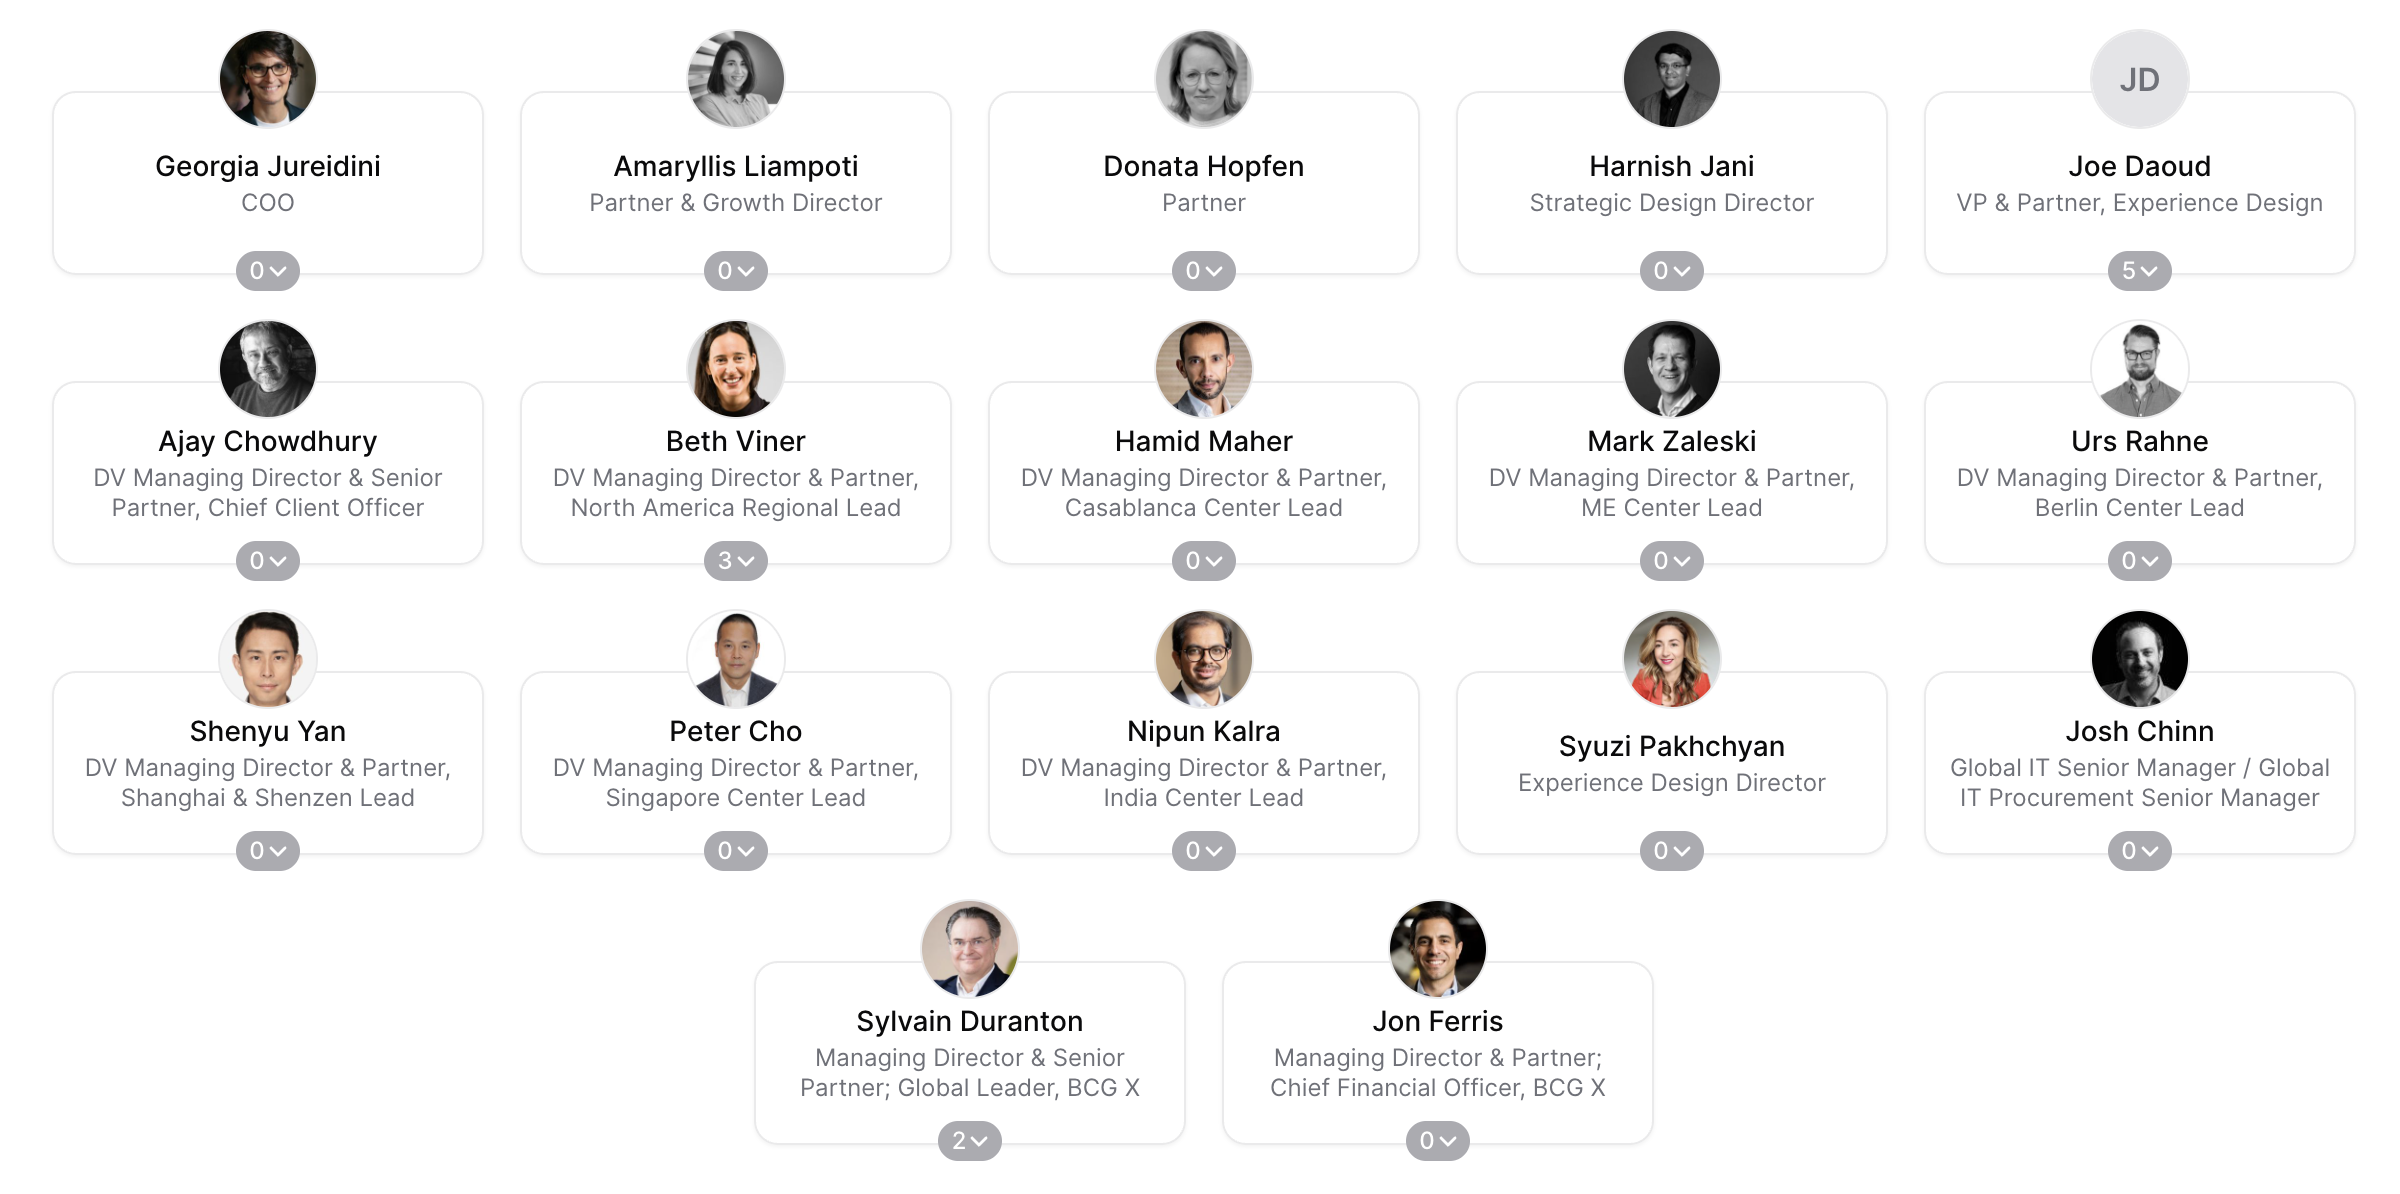
\includegraphics[width=\linewidth]{Figures/executive_leadership_board.png}
  \caption{BCG X leadership and footprint.}
  \label{fig:bcg-x-org}
\end{figure}

\subsection{Organizational Culture}

BCG~X fosters a culture defined by innovation, inclusivity, and entrepreneurial
spirit: team members are encouraged to take on ambiguous, high-impact problems and
to collaborate openly across disciplines and geographies to deliver digital
solutions for clients.

\subsection{The Energy Transition Optimizers team}
\label{sec:team}

The work presented in this report was conducted within the \textbf{Energy
Transition Optimizers} product team of BCG~X, which develops analytical products
dedicated to energy-transition projects, with a particular focus on Power-to-X
evaluation and investment-support workflows. Part of the team operates from the
BCG~X Casablanca center, alongside contributors across other geographies.

Rather than a single tool, the team maintains a small portfolio addressing
different levels of analysis: the \textbf{Energy Transition Optimizer} (the
project-level product concerned by this report), a \textbf{Portfolio Optimizer}
that compares several candidate projects under investment constraints, and a
broader \textbf{Just Energy Transition} tool that evaluates energy-transition
scenarios at a system level. This report focuses on the project-level Energy
Transition Optimizer.

The team combines product ownership, technical leadership, software engineering,
and data-oriented contributions. Figure~\ref{fig:team} summarizes its composition
and the main involvement of each member.

\begin{figure}[H]
  \centering
  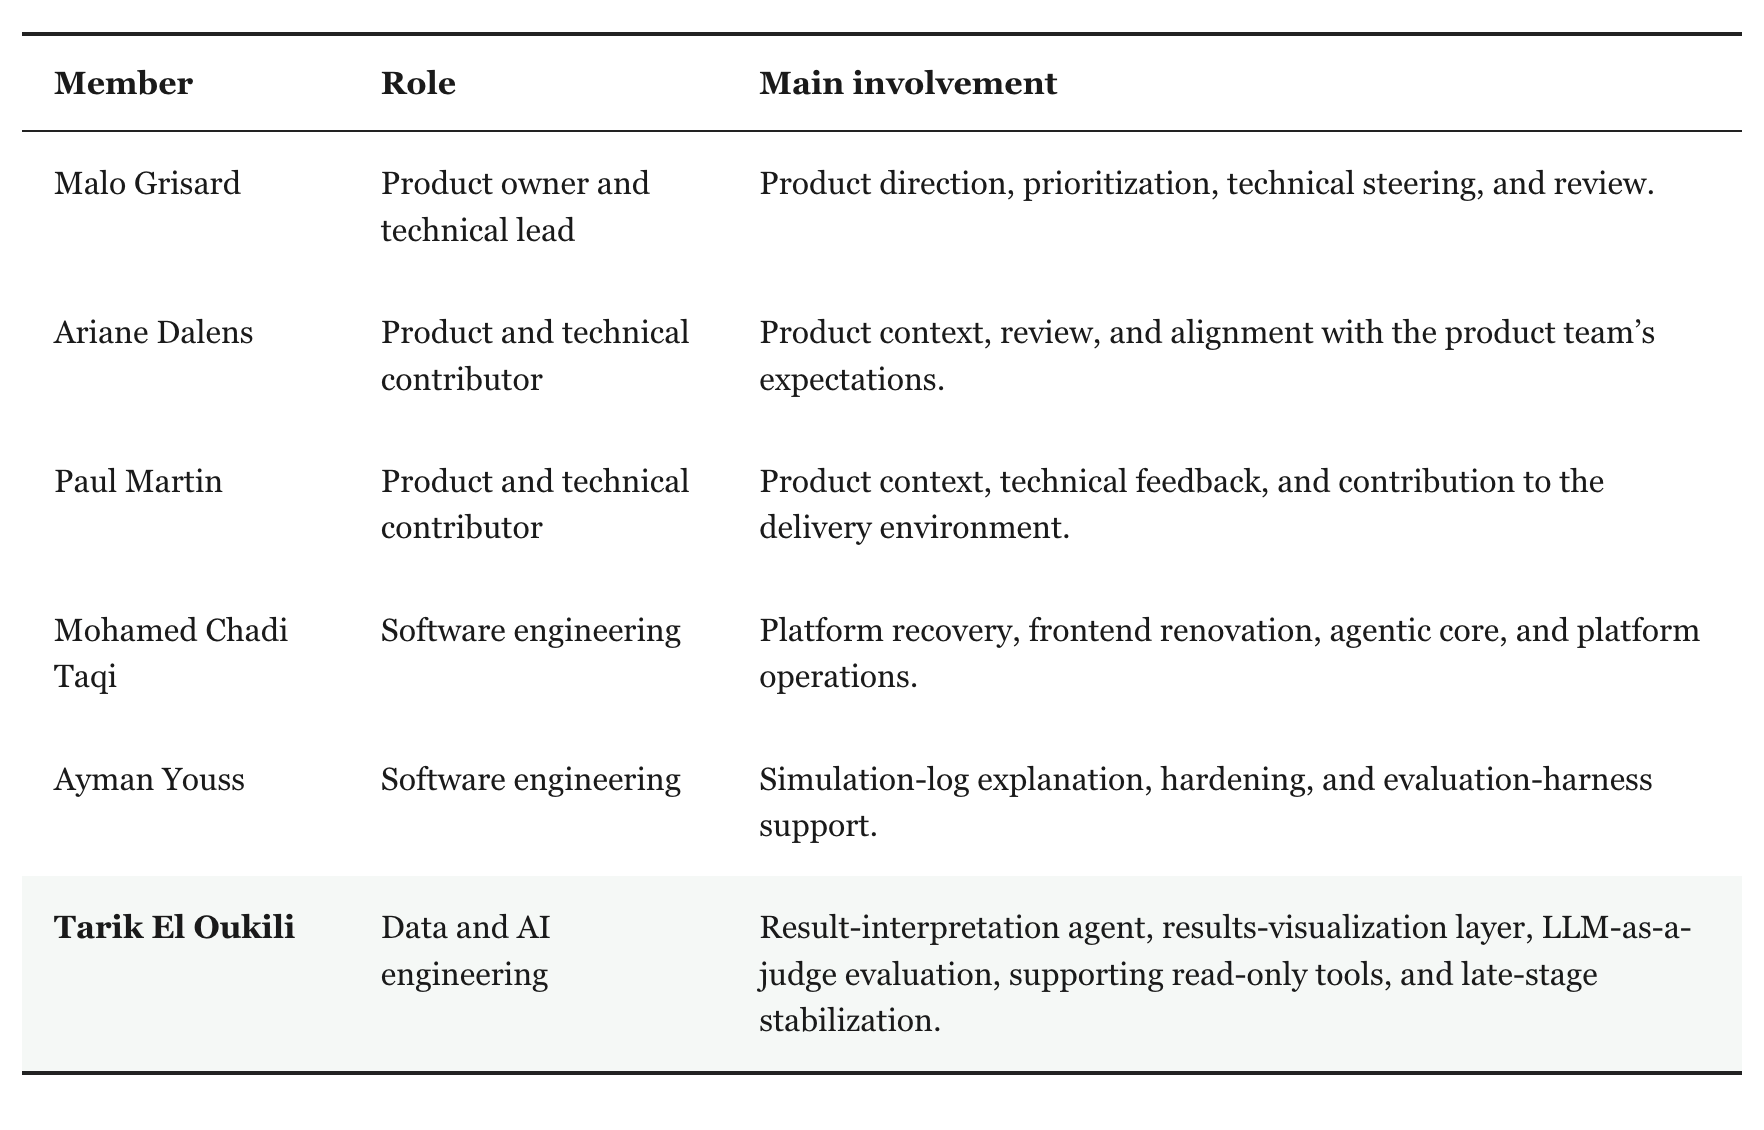
\includegraphics[width=\linewidth]{Figures/team.png}
  \caption{The Energy Transition Optimizers product team and main involvement.}
  \label{fig:team}
\end{figure}

\subsection{Internal products versus client engagements}
\label{sec:internal-product}

BCG~X delivers value through two complementary modes, and the distinction
between them shapes this entire project. In a \textbf{client engagement}, a team
builds a bespoke solution that is scoped, funded, and owned by a single client to
answer that client's specific case; the deliverable is tailored to that client
and is rarely reused as such. In an \textbf{internal product} (sometimes called
an accelerator or asset), BCG~X invests in a reusable capability that is built
and maintained in-house, and then adapted and deployed for several clients on top
of the same core.

The \textbf{Energy Transition Optimizer belongs to the second category}: it is an
internal product, not a one-off client deliverable. Several consequences follow,
and they are referenced throughout this report:

\begin{itemize}
  \item \textbf{Product-level requirements.} Reusability, maintainability,
    reproducibility, and the ability to adapt the same core to different clients
    (hence the several deployment modes described later) take precedence over the
    delivery of a single case.
  \item \textbf{Justified engineering rigor.} Continuous integration, automated
    testing, observability, and data versioning are warranted because the product
    is maintained over time and evolves across client adaptations, rather than
    being discarded at the end of an engagement.
  \item \textbf{A shared capability.} The governed multi-agent layer is designed
    as a product-level capability that lowers the barrier for \emph{every} future
    client adaptation, not as a bespoke feature for one client.
  \item \textbf{Confidentiality.} Because the product is a reusable internal
    asset, the sensitive element is never the product itself but any individual
    client that adopts it, which is the basis of the anonymization stated in
    Section~\ref{sec:confidentiality}.
\end{itemize}


\section{Internship Framework and Confidentiality}
\label{sec:confidentiality}

\begin{quote}
This internship was carried out at BCG~X, the technology and design unit of
Boston Consulting Group. To respect client confidentiality, the identity of the
end client and any customer-, site-, or counterparty-specific data have been
generalized. This anonymization does not alter the methodology, the technical
choices, or the results presented in this report.
\end{quote}

This follows directly from the operating model described in
Section~\ref{sec:internal-product}: the Energy Transition Optimizer is an
internal product rather than a client-specific deliverable. The sensitive element
is therefore never the product itself, which is described in full, but any
individual client that adopts it. Accordingly, the product, its engine, and the
governed agentic layer are presented in detail, while any specific client is
designated only as ``the client''.

\section{Energy Transition and Power-to-X}

\subsection{The decarbonization imperative}

The energy transition refers to the shift from fossil-based energy systems
toward low-carbon and renewable alternatives. While renewable electricity has
expanded rapidly, several sectors, heavy industry, aviation, maritime transport,
and high-temperature industrial processes, remain difficult to decarbonize
through direct electrification alone. For these hard-to-abate sectors,
\textbf{Power-to-X} (PtX) provides alternative energy carriers: renewable
electricity is used, most commonly through water electrolysis, to produce green
hydrogen and its derivatives (ammonia, methanol, and sustainable aviation fuel)
that can be stored, transported, and used where electrons cannot
(Figure~\ref{fig:power-to-x}).

\begin{figure}[H]
  \centering
  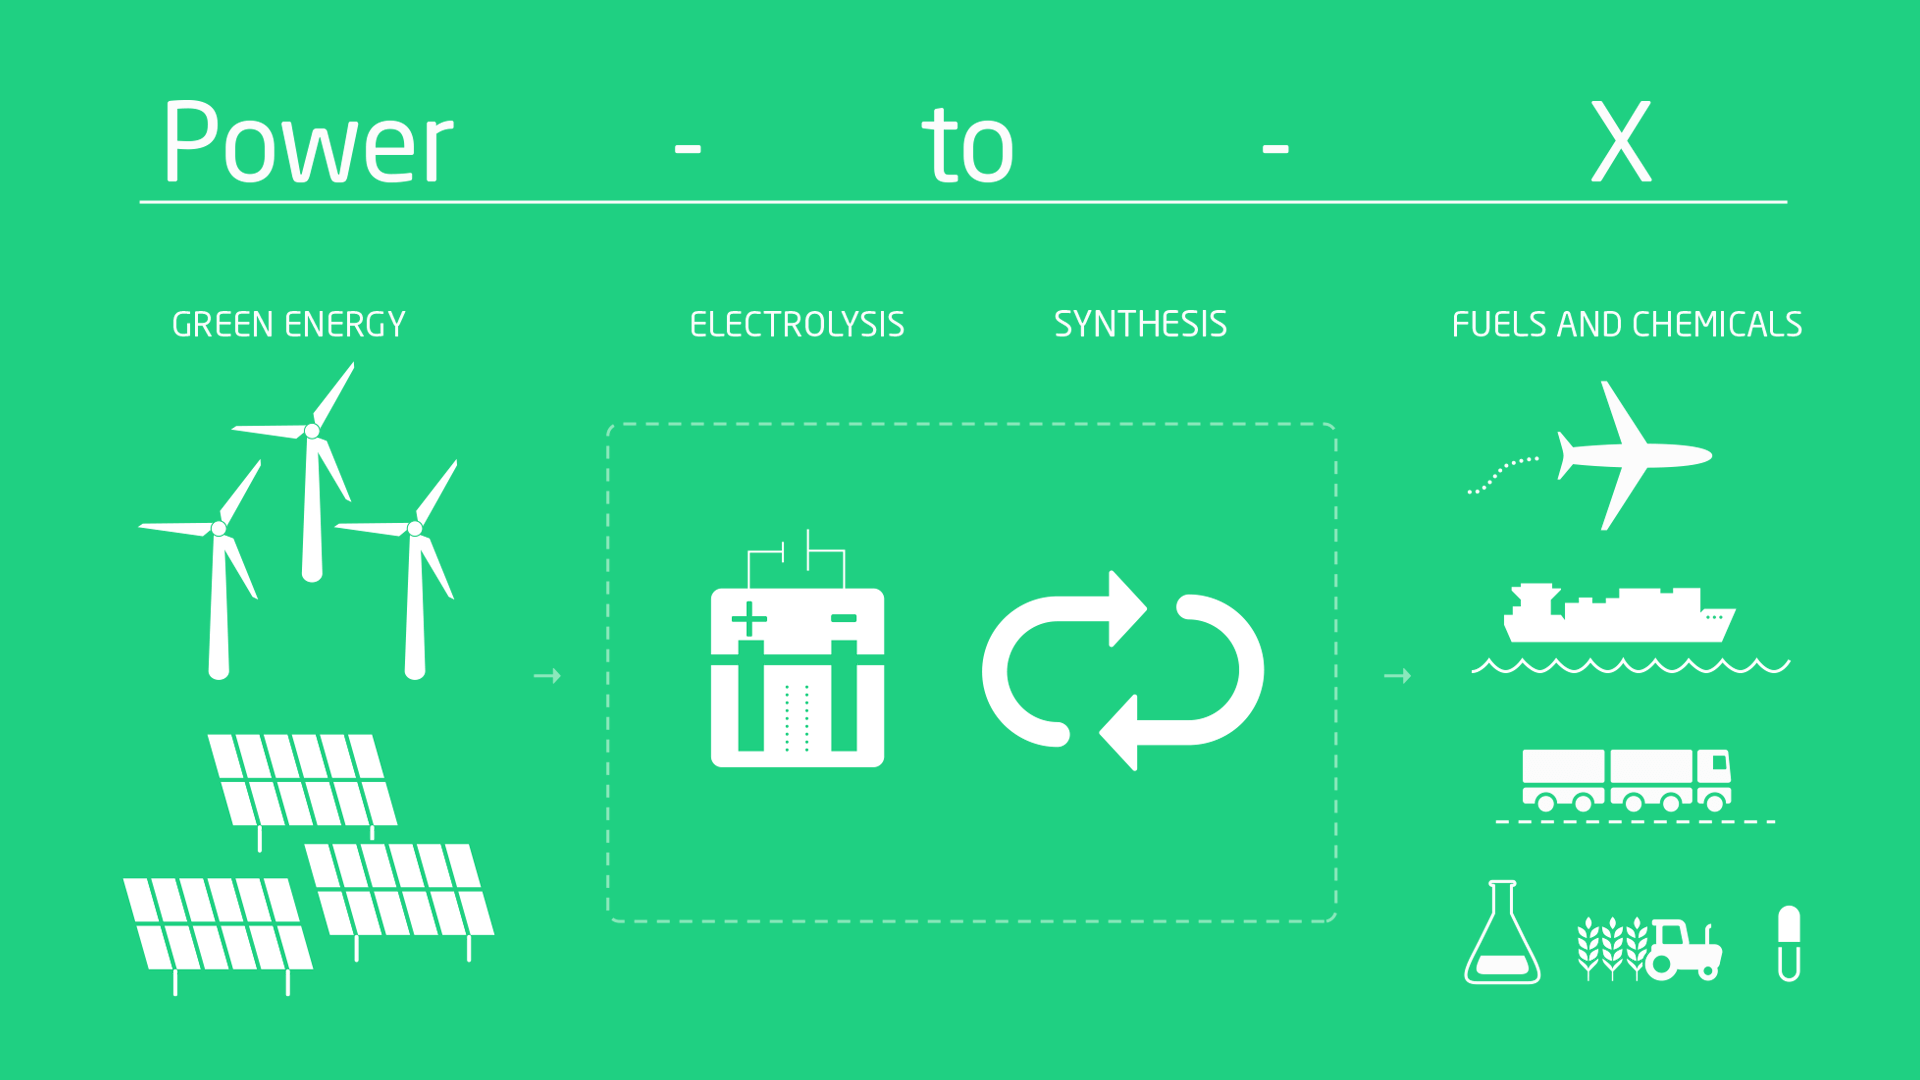
\includegraphics[width=0.8\linewidth]{Figures/power-to-x-technology.png}
  \caption{The Power-to-X principle: renewable electricity converted into
    storable, transportable energy carriers.}
  \label{fig:power-to-x}
\end{figure}



\subsection{Pre-feasibility analysis}

Power-to-X projects are capital-intensive infrastructure projects whose
development requires long planning cycles and coordination between technical,
commercial, financial, and regulatory stakeholders. The \textbf{pre-feasibility}
stage is decisive: sponsors must judge whether a project is promising enough to
justify further engineering and investment, while many assumptions remain
uncertain and cost estimates carry wide accuracy ranges. Pre-feasibility
analysis must therefore provide reliable and explainable results that help
decision-makers compare configurations, estimate economic performance, and
identify the main drivers of value and risk.

\section{The Energy Transition Optimizer}

\subsection{The product and its deterministic core}

To support this process, BCG~X developed the \textbf{Energy Transition
Optimizer} (also referred to internally as the Project Optimizer), a platform
dedicated to the pre-feasibility assessment of individual Power-to-X projects
(Figure~\ref{fig:eto-product}). It
combines a deterministic analytical core with a user-facing application.

In the engine's vocabulary, a project is described by a \textbf{topology}: a
typed directed graph whose nodes are assets (solar, wind, battery, electrolyzer,
converters, storage), commodity-conservation buses, and markets, and whose edges
represent admissible energy or material flows. Together with several hundred
technical and financial parameters (capacity factors, capital and operating
costs, the weighted-average cost of capital, escalation, and tax rates), this
topology is turned into an optimization model that simulates operation
\textbf{hour by hour} over the project's lifetime. A \textbf{grid search} sweeps
ranges of parameters to produce a population of simulations, from which the
engine reports indicators such as net present value (NPV), internal rate of
return (IRR), and the levelized cost of the output product (LCOX). Because the
results may inform investment decisions, the platform must remain reliable,
reproducible, and auditable.

\begin{figure}[H]
  \centering
  
\includegraphics[width=0.5\linewidth]{Figures/eto.png}
  \caption{The Energy Transition Optimizer product.}
  \label{fig:eto-product}
\end{figure}


\subsection{Initial situation}

Before this work began, the Energy Transition Optimizer had reached a fragile
operational state. Its analytical core remained valuable, but the surrounding
product limited its use: the workflow was expert-only, the interface was dated,
and the platform carried delivery and security weaknesses. These limitations,
which are analyzed in detail at the start of Chapter~\ref{chap:background},
motivated the two-level problem stated below.

\section{Problem Statement and Objectives}

\subsection{Problem statement}

The situation defined a two-level problem. At the \textbf{platform level}, the
product needed a restored, secure, and reproducible foundation before it could
be extended safely. At the \textbf{workflow level}, it needed to become
accessible to non-specialists without losing the rigor on which its value
depends. Meanwhile, advances in large language models opened the possibility of
a natural-language interface, but integrating such a capability into an
authoritative analytical engine raises a central tension, which frames the whole
project:

\begin{quote}
\textit{How can generative AI make an expert-only techno-economic optimizer
accessible in natural language, while preserving the reproducibility,
auditability, and human control that its results demand? In other words, how can
the assistant \emph{assist} without becoming the source of numerical truth?}
\end{quote}

\subsection{Scoping questions and expected outcomes}

This tension was broken down into a small set of scoping questions that guided the
work:

\begin{itemize}
  \item Which parts of the pre-feasibility workflow can be delegated to a language
    model, and which must remain under deterministic control?
  \item How can assisted actions be made auditable and reversible, so that a user
    can trust them and, if needed, undo them?
  \item How should the quality of a non-deterministic capability be measured
    rather than assumed?
  \item How can the same capabilities remain maintainable and adaptable across
    several client deployments?
\end{itemize}

The expected outcome was a system in which a non-specialist can design, run, and
interpret a study in natural language, where every state-changing action is
validated and approved, and where the assistant's behavior is continuously
measured, without the deterministic optimizer ever ceding its role as the source
of numerical truth.

\subsection{Objectives}
\label{sec:objectives}

The project was structured around two complementary goals. The first was to
\textbf{consolidate the platform foundation}: restore the delivery pipeline,
remediate security findings, migrate to enterprise identity, correct
infrastructure drift, renovate the interface, and improve observability. The
second was to introduce a \textbf{governed multi-agent conversational layer}: a
director agent that routes each request to specialized agents (data ingestion,
topology design, scenario exploration, and result interpretation), where every
state-changing action remains a typed proposal that is validated and then
subject to explicit human approval, so that the deterministic engine remains the
sole numerical authority.

At the heart of this effort, the agentic layer rests on three pillars,
detailed in the following chapters:

\begin{itemize}
  \item \textbf{The result-interpretation agent}: a read-only sub-agent that
    explains the economics of a simulation population in natural language, with
    every figure traceable back to a deterministic result and no invented
    numbers.
  \item \textbf{The results-visualization layer}: interactive exploration of
    outputs, including interpret-on-demand scatter plots and a navigable
    discounted-cash-flow table.
  \item \textbf{The evaluation harness}: an ``LLM-as-a-judge'' mechanism that
    measures the factual grounding and financial soundness of the explanations
    produced.
\end{itemize}

Methodologically, the work followed the arc of a design-oriented engineering
project rather than a controlled experiment: it identifies the problem and its
constraints (this chapter), reviews the state of the art and chooses a direction
(Chapter~\ref{chap:background}), specifies the requirements
(Chapter~\ref{chap:requirements}), designs and builds the artifacts
(Chapter~\ref{chap:design}), demonstrates them in the delivered product, and
evaluates the assisted behavior against explicit criteria
(Chapter~\ref{chap:implementation}), with the limits of that evaluation stated
rather than hidden. This progression structures the chapters that follow.

\section{Project Management}

\subsection{Agile delivery approach}

The project followed an agile delivery approach adapted to a product-modernization
effort. Rather than fixed sprint boundaries, the work progressed through short
delivery cycles and overlapping thematic phases: the platform foundation was
consolidated first, the governed agentic core was introduced next, specialist
capabilities (including result interpretation) were then extended, and a final
phase focused on observability, hardening, and handover. Priorities were adjusted
as the dependencies between infrastructure, security, and the agentic layer became
clearer, while continuous integration and regular review with the product team
kept the application deployable throughout. My own work followed the same rhythm,
moving from the visualization layer to the interpreter agent and its evaluation,
as shown in the timeline at the end of this section. Within each phase, the work
iterated through the classic agile cycle of requirements, design, development,
testing, deployment, and review (Figure~\ref{fig:agile-cycle}).

\begin{figure}[H]
  \centering
  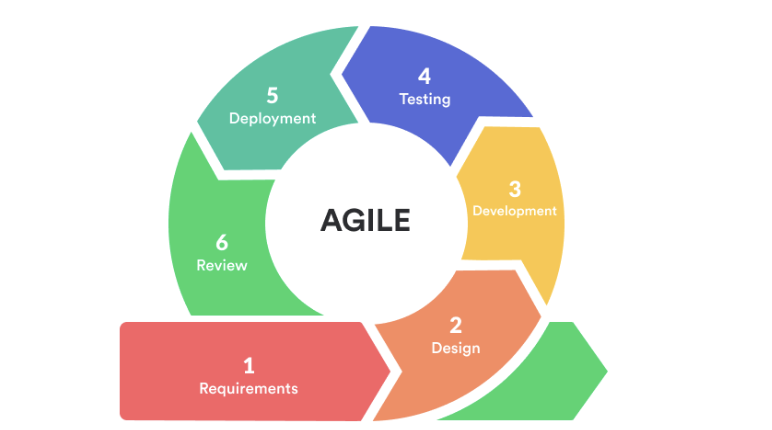
\includegraphics[width=0.62\linewidth]{Figures/agile_cycle.png}
  \caption{The agile delivery cycle followed within each thematic phase.}
  \label{fig:agile-cycle}
\end{figure}

\subsection{Working cadence}

The internship followed the standard cadence of a BCG engagement, built around a
small set of recurring meetings:

\begin{itemize}
  \item \textbf{Daily check-in} in the morning to align on the day's priorities
    and any blockers.
  \item \textbf{Daily check-out} in the afternoon to review progress and hand
    off open items.
  \item \textbf{Case Team Meeting} once a week with the engagement
    Managing Directors and Partners, focused on direction, risks, and key
    decisions.
  \item \textbf{Monthly retrospective} to reflect on what worked, what did not,
    and how to improve.
\end{itemize}
\subsection{Collaboration tools}

The engagement used a small, shared set of tools. Most supported communication
and coordination across the wider team; the technical team additionally used
GitHub, with CircleCI for continuous integration, for code review and delivery.

\begin{itemize}\itemsep=10pt
  \item \textbf{Zoom} and \textbf{Microsoft Teams}: video and audio calls, daily
    check-ins and check-outs, Case Team Meetings, and engagement-wide channels.\\[5pt]
    \mbox{}\hfill
\includegraphics[height=1.9cm]{Logos/zoom.png}\hspace{1.6em}%
    
\includegraphics[height=1.9cm]{Logos/teams.png}\hfill\mbox{}
  \item \textbf{Trello}: a kanban board tracking work items, each card carrying an
    owner, a status, and a short description.\\[5pt]
    \mbox{}\hfill
\includegraphics[height=1.9cm]{Logos/trello.png}\hfill\mbox{}
  \item \textbf{Slack}: lightweight, asynchronous chat within the technical team.\\[5pt]
    \mbox{}\hfill
\includegraphics[height=1.9cm]{Logos/slack.png}\hfill\mbox{}
  \item \textbf{Outlook}: email and calendar management for the recurring
    meetings.\\[5pt]
    \mbox{}\hfill
\includegraphics[height=1.9cm]{Logos/outlook.png}\hfill\mbox{}
  \item \textbf{GitHub}: code hosting and pull-request review, with CircleCI
    running continuous-integration checks on every change.\\[5pt]
    \mbox{}\hfill
\includegraphics[height=1.9cm]{Logos/github.png}\hfill\mbox{}
\end{itemize}

\subsection{Timeline and milestones}

The internship ran from \textbf{June to September 2026}. My work followed the plan
shown in Figure~\ref{fig:gantt}, organized into two overlapping phases that moved
from the results-visualization layer to the interpreter agent and its evaluation.

\textbf{Phase~1 (visualization and financials)} covered the results-visualization
layer: interactive results exploration, chart user-experience and polish, the
drillable discounted-cash-flow (DCF) financials table, and a consolidating
refactor of the visualization and financial components.

\textbf{Phase~2 (interpreter and evaluation)} built the result-interpretation
agent and the means to evaluate it: the interpreter sub-agent, its narration
prompt and grounding rules, Langfuse tracing and datasets, the LLM-as-a-judge
rubrics, a refactor of the agent and evaluation code, and a final feedback loop
and demonstration preparation.

\begin{figure}[H]
  \centering
  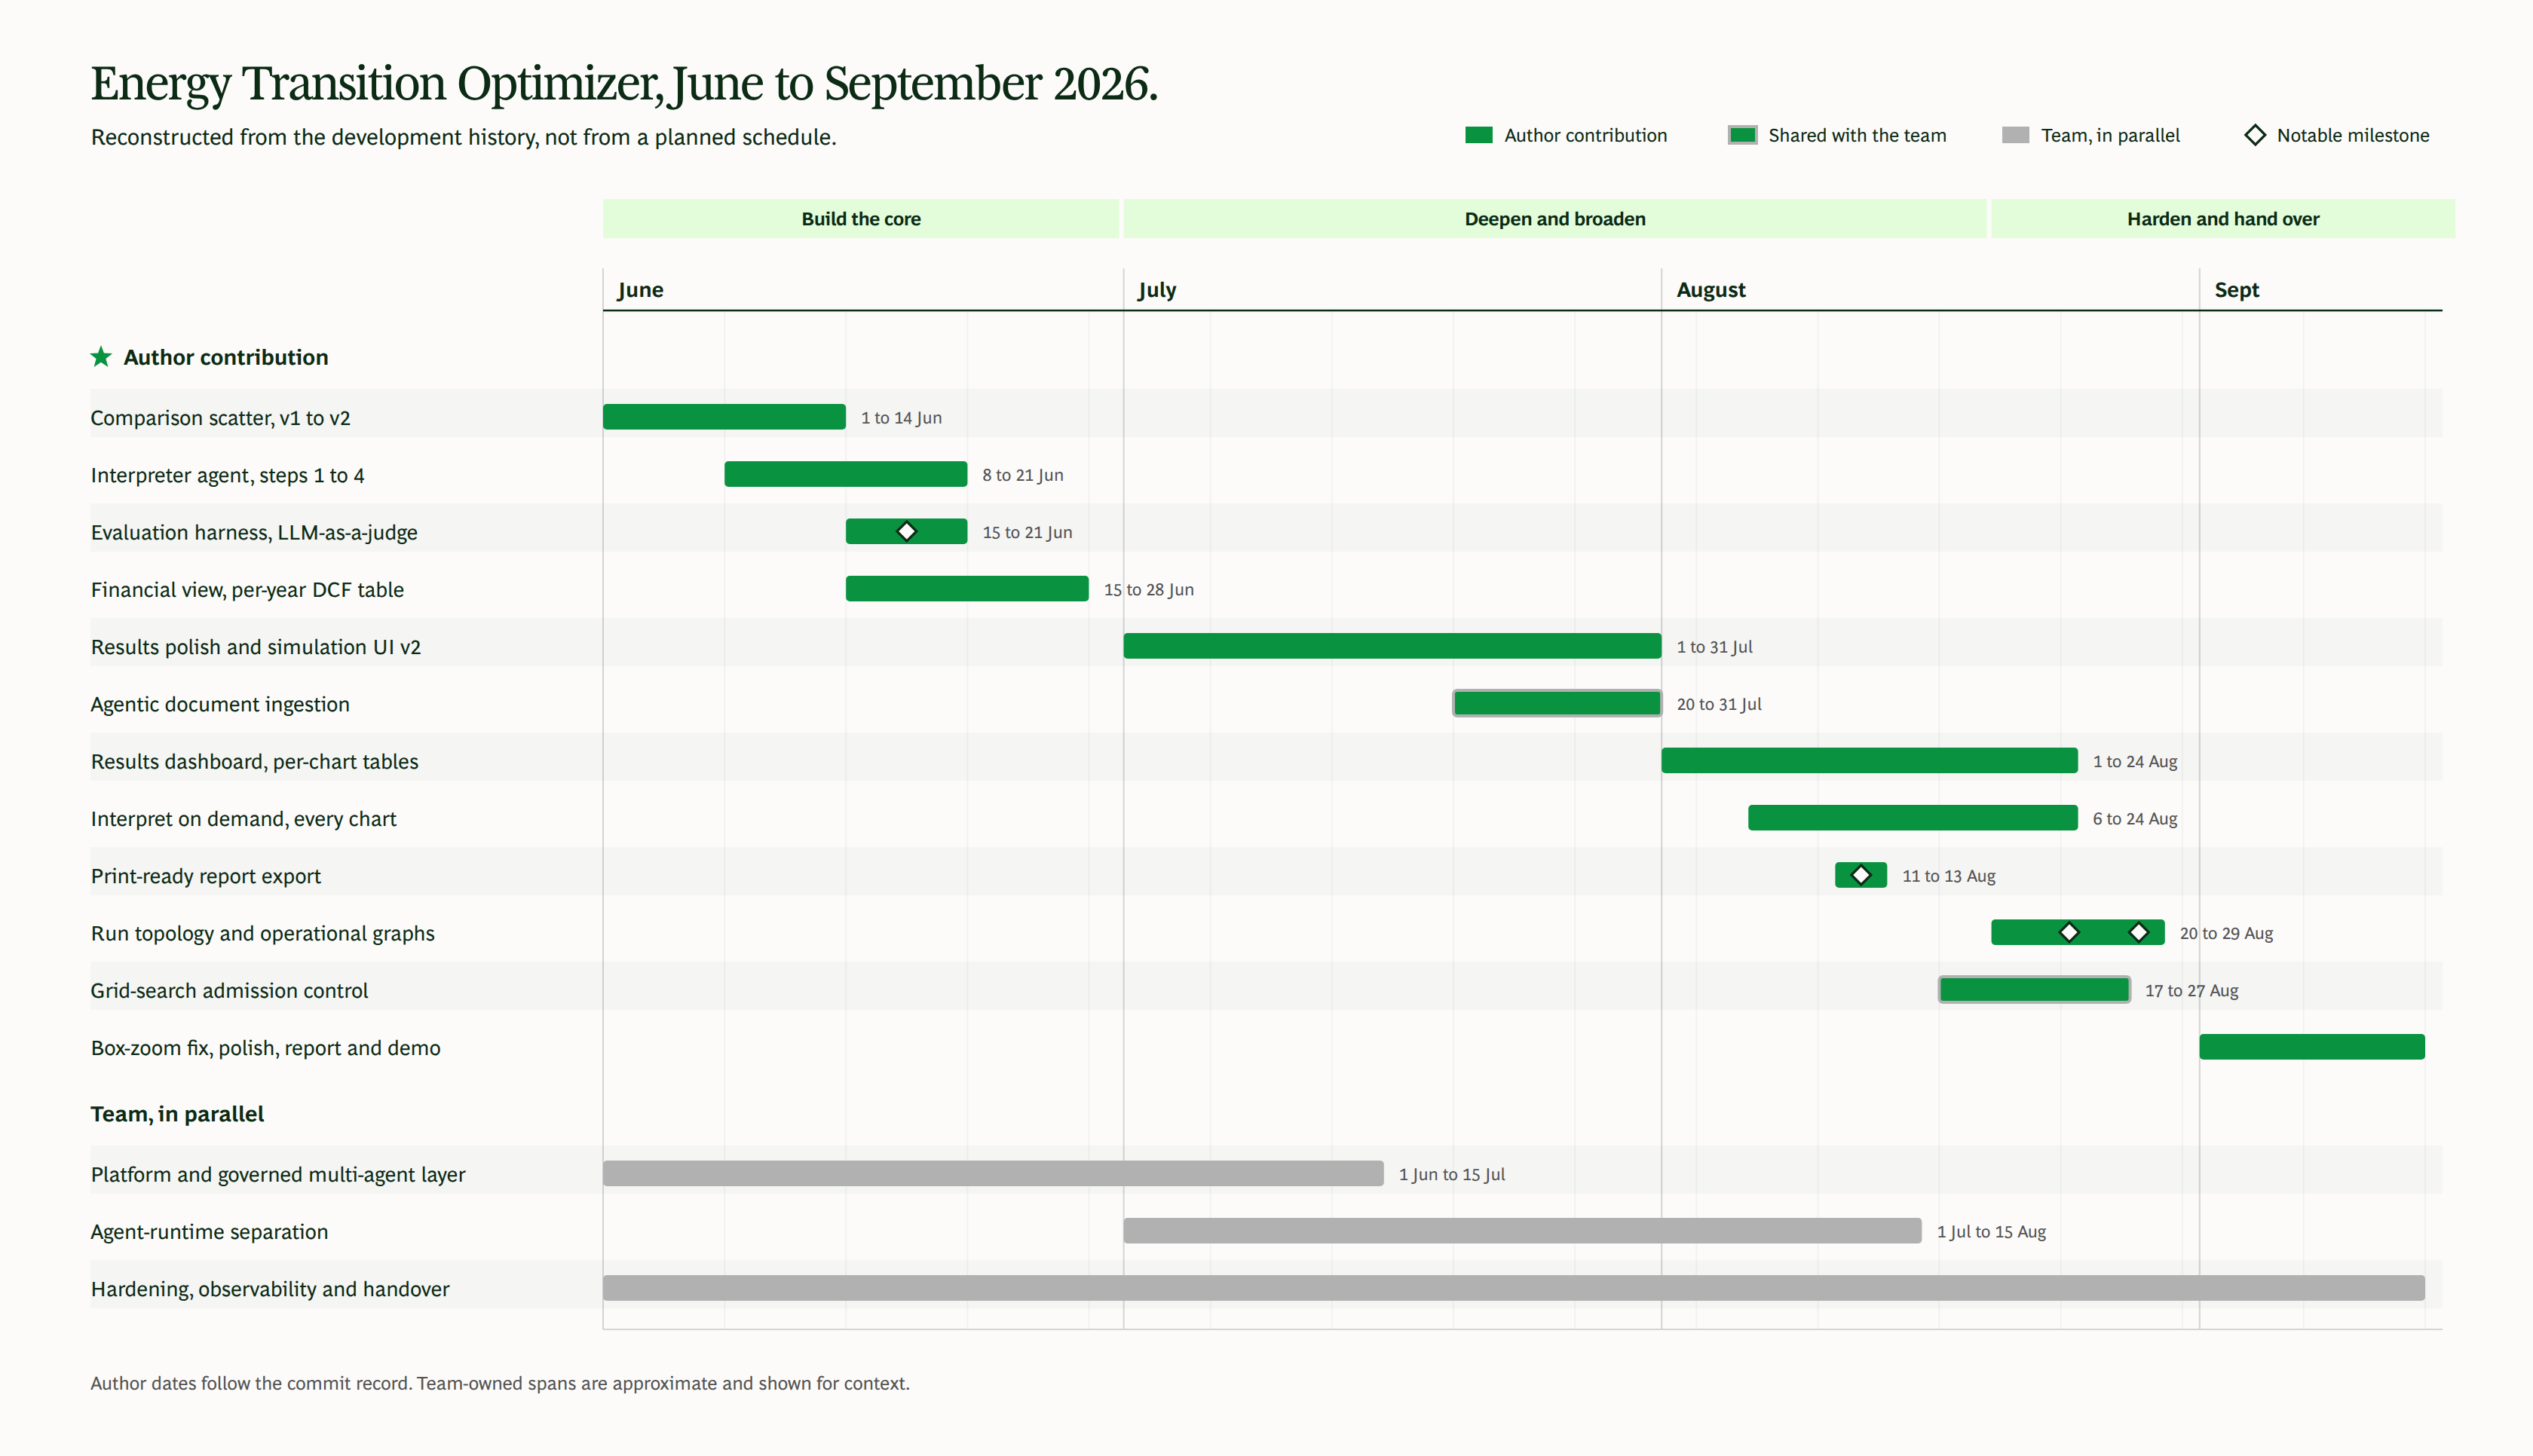
\includegraphics[width=\linewidth]{Figures/optimizer-timeline.png}
  \caption{Internship work plan (June--September 2026).}
  \label{fig:gantt}
\end{figure}

\section*{Conclusion}

This chapter introduced the host organization, the Energy Transition Optimizers
product team, and the energy-transition context of the project. It presented the
Energy Transition Optimizer, its fragile initial state, and the two-level problem
the internship addressed, and it framed the central tension between accessibility
and numerical authority. The next chapter reviews the technical background and
state of the art on which the work rests.
